\documentclass[14pt,a4paper]{scrartcl}
\usepackage[utf8]{inputenc}
\usepackage{ragged2e}
\usepackage{xcolor}
\usepackage[english,russian]{babel}
\usepackage{misccorr,color,ragged2e,amsfonts,amsthm,graphicx,systeme,amsmath,mdframed,lipsum}
\renewcommand\qedsymbol{$\blacksquare$}
\renewcommand*{\proofname}{\text{Доведення}}
\theoremstyle{definition}
\newtheorem{defo}{Означення}[section]
\newtheorem*{teo}{Теорема}
\newtheorem*{example}{Приклад}
\theoremstyle{remark}
\newtheorem*{remark}{Зауваження}
\theoremstyle{definition}
\newtheorem*{consequence}{Наслідок}
\theoremstyle{definition}
\newtheorem{statement}{Утверждение}[section]
\newmdtheoremenv{boxteo}{Теорема}[section]
\setlength\parindent{0pt}
\DeclareMathOperator*\lowlim{\underline{lim}}
\DeclareMathOperator*\uplim{\overline{lim}}


% Default fixed font does not support bold face
\DeclareFixedFont{\ttb}{T1}{txtt}{bx}{n}{12} % for bold
\DeclareFixedFont{\ttm}{T1}{txtt}{m}{n}{12}  % for normal

% Custom colors
\usepackage{color}
\definecolor{deepblue}{rgb}{0,0,0.5}
\definecolor{deepred}{rgb}{0.6,0,0}
\definecolor{deepgreen}{rgb}{0,0.5,0}

\usepackage{listings}

% Python style for highlighting
\newcommand\pythonstyle{\lstset{
language=Python,
basicstyle=\ttm,
otherkeywords={self},             % Add keywords here
keywordstyle=\ttb\color{deepblue},
emph={MyClass,__init__},          % Custom highlighting
emphstyle=\ttb\color{deepred},    % Custom highlighting style
stringstyle=\color{deepgreen},
frame=tb,                         % Any extra options here
showstringspaces=false            %
}}

\definecolor{javared}{rgb}{0.6,0,0} % for strings
\definecolor{javagreen}{rgb}{0.25,0.5,0.35} % comments
\definecolor{javapurple}{rgb}{0.5,0,0.35} % keywords
\definecolor{javadocblue}{rgb}{0.25,0.35,0.75} % javadoc

\lstset{language=C++,
basicstyle=\ttfamily,
keywordstyle=\color{javapurple}\bfseries,
stringstyle=\color{javared},
commentstyle=\color{javagreen},
morecomment=[s][\color{javadocblue}]{/**}{*/},
numbers=left,
numberstyle=\tiny\color{black},
stepnumber=2,
numbersep=10pt,
tabsize=4,
showspaces=false,
showstringspaces=false}


% Python environment
\lstnewenvironment{python}[1][]
{
\pythonstyle
\lstset{#1}
}
{}

% Python for external files
\newcommand\pythonexternal[2][]{{
\pythonstyle
\lstinputlisting[#1]{#2}}}

% Python for inline
\newcommand\pythoninline[1]{{\pythonstyle\lstinline!#1!}}
%
% \begin{python}
% class MyClass(Yourclass):
%     def __init__(self, my, yours):
%         bla = '5 1 2 3 4'
%         print bla
% \end{python}

\begin{document}



\def\be{\begin{equation}}
\def\ee{\end{equation}}
\def\bd{\begin{defo}}
\def\ed{\end{defo}}
\def\bbt{\begin{boxteo}}
\def\ebt{\end{boxteo}}
\begin{center}
Розрахункова робота № 1 \\
	Терещенко Денис КА-96 \\
	Варіант - 27
\end{center}

2.27. Розв'язати задачу Коші. У вигляді системи:
$$
\left\lbrace
\begin{gathered}
ydx + (2x - 2 \sin^2{(y)} - y \sin{(2y)}  )dy = 0\\
y(3/2) = \frac{\pi}{4}
\end{gathered}
 \right.
$$
Перейдемо від рівняння Пфаффа до зручного вигляду лінійного рівняння. Але, розв'язок будемо шукати відносно змінної $x$:
$$
\left\lbrace
\begin{gathered}
\color{blue}
x' + \frac{2x}{y} - \frac{2 \sin^2{(y)} }{y} - \sin{(2y)} = 0\\
x(\frac{\pi}{4}) = 3/2
\end{gathered}
 \right.
$$
Прийшли до лінійного рівняння, для якого скористаємося методом Бернуллі:
$$
x(y) = v(y)\cdot u(y) =vu
$$
$$
uv' + vu' + \frac{2uv}{y} - \frac{2 \sin^2{(y)} }{y} - \sin{(2y)} =0
$$
$$
uv' + v (u' + \frac{2u}{y} ) - \frac{2 \sin^2{(y)} }{y} - \sin{(2y)} =0
$$
Розв'яжемо відносно $u$:
$$
\color{blue}
\begin{gathered}
  u' + \frac{2u}{y} = 0\\
	\ln{u} = -2 \ln{y} + C_u
\end{gathered}
 \quad \Longrightarrow \quad
 \begin{gathered}
  C_u = 0 \\
	u = \frac{1}{y^2}
 \end{gathered}
$$
$$
y^{-2}v'  - \frac{2 \sin^2{(y)} }{y} - \sin{(2y)} =0
$$
$$
v =  \int\limits_{}^{}{\frac{2 \sin^2{(y)} }{y} + \sin{(2y)}dy} = y^2 \sin^2{(y)} + C
$$
$$
x(y) = u*v = \sin^2{y} + \frac{C}{y^2}
$$
Далі повернемося до задачі Коші, підставляючи числа:
$$
1 = \frac{16C}{ \pi^2} \Longrightarrow C = \frac{\pi^2}{16}
$$

\pagebreak

3.27. Знайти розв'язок задачі Коші. Запишемо у вигляді системи:
$$
\left\lbrace
\begin{gathered}
 y'  + y = xy^2\\
  y(0) = 1
\end{gathered} \right.
$$
Розв'яжемо за методом Бернуллі:
$$
\begin{gathered}
\text{Заміна:}\\
y(x) = v(x)\cdot u(x) = vu
\end{gathered}
\quad \Longrightarrow \quad
\begin{gathered}
 uv' + vu' + uv - xu^2v^2 = 0 \\
 uv' + v(u' + u) - xu^2v^2 = 0
\end{gathered}
$$
Знайдемо $u$ з умови $u' + u =0$:
$$
u' + u =0 \qquad  \int\limits_{}^{}{ \frac{1}{u} du}  =  -\int\limits_{}^{}{1 dx} \Big|_{C=0} \qquad \ln{ \left| u \right| } = -x \Longrightarrow u = e^{-x}
$$
$$
e^{-x}v' = v^2 \cdot e^{-2x}
$$
$$
 \int\limits_{}^{}{ \frac{dv}{v^2} } =  \int\limits_{}^{}{ x e^{-x}dx }
$$
$$
\int\limits_{}^{}{ x e^{-x}dx } = \left| \begin{gathered}
 d\mu =  e^{-x} \\
 \nu = x \qquad dx = d\nu\\
 \mu =  - e^{-x}
\end{gathered} \right| = -xe^{-x} -e^{-x} = -e^{-x} (x+1) + C
$$
$$
y = \frac{e^{-x}}{ e^{-x} (x+1) +C} = \frac{1}{x+1 + Ce^{-x}}
$$
Підставляючи відповідні значення з умови задачі Коші:
$$
1 = \frac{1}{ 0 + C + 1}  \Longrightarrow  C = 0 \Longrightarrow y = \frac{1}{x+1}
$$

\pagebreak

4.27. Знайти лінію, що проходить через точку $M_0$ та має властивість, що в будь-який її точці $M$ дотичний вектор $\overline{MN}$ з кінцем на осі $Oy$ має проекцію на вісь $Oy$, рівну a.
$$
\begin{gathered}
\text{Умова:}\\
M_0 (1,4)\\
  a = 2
\end{gathered}
 \qquad \qquad
\begin{gathered}
  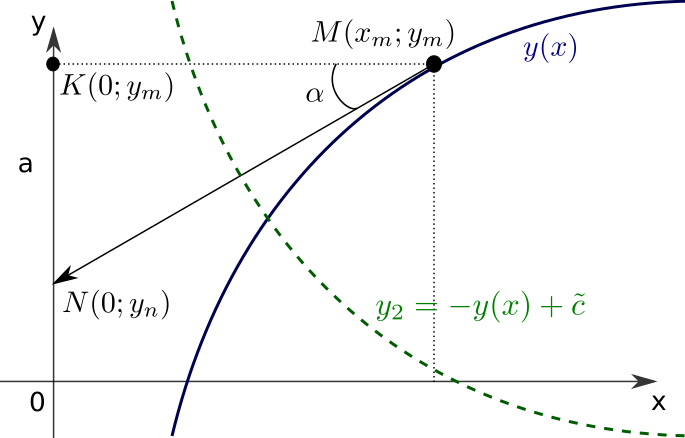
\includegraphics[scale=0.32]{1.png}
\end{gathered}
$$
Спочатку розглянемо вектор $ \overline{MN}$, для якого знаємо, що $N(0, y_n)$. Опустимо нормаль з точки $M(x_m, y_m)$ до $Oy$ - отримаємо т. $K(0, y_n -a)$.
З геометричного змісту похідної та $\triangle KMN(KM=x;KN=a; \angle{KMN}  = \alpha)$, отримаємо вираз для $a$:
$$
a = x_m \cdot \tg{(\alpha)} = x_m y'(x_m)
$$
Ми розглядаємо лише додатні значення похідної, тобто $y(x)$ ми знайдемо як зростаючу функцію. Однак розв'язком також буде функція $y_2(x) = - y(x)$, для якої проекія також буде дорівнювати $a$. Також, попередньо можна сказати, що функція буде або показниковою, або логаріфмічною. Прийшли до задачі Коші:
$$
\left\lbrace
\begin{gathered}
 y'x = 2 \\
 y(1) = 4
\end{gathered}
 \right.
$$

$$
\begin{gathered}
 y' = \frac{2}{x}\\
 y =  \int\limits_{}^{}{ \frac{2}{x}dx } \\
 y = 2\ln{ \left| x \right| } + C \\
\end{gathered}
\qquad
\qquad
\qquad
\begin{gathered}
\text{Але, пам'ятаємо, що існують}\\
\text{розв'язки, симетричні за } Ox \\
y_1 = 2\ln{x} + C_1 \\
y_2 = -2\ln{x} + C_2
\end{gathered}
$$

Підставивши значення з умови задачі Коші:

$$
C_1 = C_2 = 4 \Longrightarrow \begin{gathered}
y_1 = 2\ln{x} + 4\\
y_2 = -2\ln{x} +4
\end{gathered}  \quad I = (0,  +\infty)
$$

\pagebreak

5.27. Знайти розв'язок задачі Коші.

$$
y''y^3 + 4 = 0 \qquad y(0) = -1 \qquad y'(0) = -2
$$

У рівнянні відсутні доданки, залежні від $x$, тож скористаємося заміною:

$$
z(y) = y' \Longrightarrow y'' = z * z'
$$
$$
\left\lbrace \begin{gathered}
z' * z = \frac{4}{y^3}\\
z(-1) = -2
\end{gathered} \right.
 \qquad  \int\limits_{}^{}{zdz} = -4  \int\limits_{}^{}{ \frac{dy}{y^3} }
$$
$$
z^2 = \frac{4}{y^2} + C_1 \qquad \text{або} \qquad z = \pm \sqrt{ \frac{4}{y^2} +C_1 }
$$

Розглядаємо $z(y)$ в околі т. $-1$, тож $ -2 = - \sqrt{ 4 + C_1} \Longrightarrow C_1 = 0$. Отримали:

$$
z = - \frac{2}{ \left| y \right| } \qquad y \in U_{\varepsilon}(-1) \Longrightarrow \begin{gathered}
 \left| y \right| = -y \\
 z = \frac{2}{y}
\end{gathered} \Longrightarrow y' = \frac{2}{y}
$$

$$
yy' = 2; \quad ydy = 2dx; \quad \frac{y^2}{2} = 2x+C_2; \quad y = \pm\sqrt{ 4x +C }
$$

Підставимо $y =-1 \quad x = 0$. Знайшли параметр $С$: $C=1 \Longrightarrow \mathbf{y = - \sqrt{4x+1}}$

\pagebreak

6. 27. Знайти загальний розв'язок диференціального рівняння.

\be
y''' - 64y' = 128 \cos{(8x)} - 64e^{8x}
\ee

Розв'яжемо відповідне однорідне рівняння:

$$
y''' - 64y' = 0
$$

Характеристичне рівняння:

$$
\lambda( \lambda^2 - 64) = 0 \quad \Longrightarrow \quad \begin{gathered}
 \lambda = \pm 8;0
\end{gathered}
$$

Отримали загальний розв'язок:

$$
y_{\text{з.о}} = C_1e^{-8x} + C_2e^{8x} + C_3
$$

Для рівняння (1) роз'язок $y = y_{\text{ч}} + y_{\text{з.о}}$. $y_{\text{ч}}$ знайдемо користуючись принципом суперпозиції:
$$
\left(
\begin{gathered}
y_1 - \text{ част. розв. } y''' - 64y'  = 128 \cos{(8x)} \\
y_2 - \text{ част. розв. } y''' - 64y'  = - 64e^{8x}\\
y_{\text{ч}} = y_1 + y_2
\end{gathered} \right)
 \Leftrightarrow y_{\text{ч}}  - \text{ част. розв. рівняння (1) }
$$
$y_1$ шукаємо у вигляді $A \sin{(8x)} + B \cos{(8x)}  $:
$$
y_1' = 8(A\cos{(8x)}  - B\sin{(8x)} )
$$
$$
y_1''' = 512(B \sin{(8x)} - A\cos{(8x)} )
$$
$$
512( B\sin{(8x)} -A \cos{(8x)} ) - 512 (A\cos{(8x)}  - B\sin{(8x)} )  = 128 \cos{(8x)}
$$
$$
1024 A \cos{(8x)} = - 128 \cos{(8x)} \Longrightarrow  B =0  \quad A = - \frac{1}{8}
$$
$y_2$ шукаємо у вигляді $e^{8x}(Ax)$:
$$
y_2' = Ae^{8x} + 8Axe^{8x}
$$
$$
y_2''' = 192 A e^{8x} + 512 A x e^{8x}
$$
$$
192 A e^{8x} + 512 A x e^{8x} - 64(Ae^{8x} + 8Axe^{8x}) = -64e^{8x}
$$
$$
192 A - 64 A = -64  \Longrightarrow A = -\frac{1}{2}
$$
Таким чином, можемо записати розв'язок рівняння(1):
$$
y = C_1e^{-8x} + C_2e^{8x} + C_3 - \frac{1}{8}\sin{(8x)} - \frac{1}{2} xe^{8x}
$$

\pagebreak

7.27. Знайти розв'язок задачі Коші.
$$
y'' + y = 2 \ctg{(x)} \qquad y( \pi/2) = 1 \qquad y'(\pi/2) = 2
$$
Розглянемо відповідне однорідне рівняння $y'' + y = 0$. \\
Його характеристичне рівняння $\lambda^2 + 1 = 0 \Rightarrow \lambda = \pm i$.
$$
y_{\text{з.о.}} (x) = C_1 \cos{(x)} + C_2 \sin{(x)}
$$
Cкористаємося методом варіації: шукаємо розв’язок неоднорідного диф.рівняння у вигляді $ y_{\text{з.о.}} (x) = C_1(x) \cos{(x)} + C_2(x) \sin{(x)}   $, де $C_1 ( x ), C_2 ( x )$ повинні задовольняти системі:
$$
\left\lbrace
\begin{gathered}
 C_1'(x) \cos{(x)} + C_2'(x) \sin{(x)} =0 \\
 - C_1'(x) \sin{(x)} + C_2'(x)\cos{(x)} = 2 \ctg{x}
\end{gathered}
 \right.
 \Leftrightarrow
 \left\lbrace
 \begin{gathered}
  C_1'(x) \cos{(x)} + C_2'(x) \sin{(x)} =0 \\
  - C_1'(x) \frac{\sin^2{(x)}}{ \cos{(x)} }  + C_2'(x)\sin{(x)} = 2
 \end{gathered}
  \right.
$$
$$
\Leftrightarrow
\left\lbrace
\begin{gathered}
 C_1'(x) (\cos{(x)} + \frac{\sin^2{(x)}}{ \cos{(x)} }) = -2\\
 C_2'(x) = \frac{2}{ \sin{(x)} } - \sin{(x)}
\end{gathered}
 \right.
 \Leftrightarrow
 \left\lbrace
 \begin{gathered}
 C_1'(x) = -2 \cos{(x)}\\
 C_2'(x) =  2\ctg{(x)} \cdot \cos{(x)}
 \end{gathered}
  \right.
$$
Проінтегрувавши, отримаємо:
$$
C_1 = -2 \sin{(x)} + C^*_1 \qquad C_2 = 2 \cos{(x)} + 2 \ln{ \tg{\Big( \frac{x}{2} \Big)} } + C^*_2
$$
Отримали розв'язок диф.рівняння:
$$
y = -2 \sin{(x)} \cos{(x)} + C^*_1 \cos{(x)} + 2 \cos{(x)}\sin{(x)} + 2 \ln{\tg{\Big( \frac{x}{2} \Big)} }\sin{(x)} + C^*_2 \sin{(x)}
$$
\begin{center}
\fbox{$
y = C^*_1 \cos{(x)} + 2 \ln{\tg{\Big( \frac{x}{2} \Big)} }\sin{(x)} + C^*_2 \sin{(x)}
$}
\end{center}
$$
y' = -C_1^*\sin{(x)} + 2 + C_2 \cos{(x)}
$$
Підставивши значення з умови задачі Коші:
$$
\left\lbrace
\begin{gathered}
 1 = 0 + 0 + C^*_2\\
 2 = - C^*_1 + 2 + 0
\end{gathered} \right.  \quad \Longrightarrow \quad
\left\lbrace
\begin{gathered}
  C_1^* =0\\
	C_2^* = 1
\end{gathered}
 \right.
$$
Остаточно, розв'язок задачі Коші:
\begin{center}
\fbox{
$y = 2 \ln{\tg{\Big( \frac{x}{2} \Big)} }\sin{(x)} + \sin{(x)}$
}
\end{center}

\pagebreak

8.27. Розв'язати систему диф.рівнянь.

$$
\left\lbrace
\begin{gathered}
 x' = -x + y + z + 2t \\
 y' = -5x + 21 y = 17z + 3\\
 z' = 6x - 26y - 21z -t^2
\end{gathered} \right.
$$
Спочатку знайдемо розв'язок відповідної однорідної системи:
$$
\left\lbrace
\begin{gathered}
 x' = -x + y + z\\
 y' = -5x + 21 y + 17z\\
 z' = 6x - 26y - 21z
\end{gathered} \right.
$$
Запишемо матрицю системи:
$$
A = \begin{bmatrix}
 -1 & 1 & 1 \\
 -5 & 21 & 17 \\
 6 & -26 & -21
\end{bmatrix}
$$
Знайдемо фундаментальну матрицю $Y = e^{tA} = U e^{tA} U^{-1}; A = U \Lambda U^{-1}$.

Знайдемо власні числа матриці:
$$
\det (A  - \lambda  I ) = \begin{vmatrix}
-1 - \lambda & 1 & 1 \\
-5 & 21 - \lambda & 17 \\
6 & -26 & -21- \lambda
\end{vmatrix}=
$$
$
 =  ( 1 + \lambda) ( 21 - \lambda) ( 21 - \lambda) + 17\cdot 6 -130 - 6 ( -\lambda + 21  ) - 26\cdot 17 ( - \lambda - 1 ) -5 ( \lambda + 21) =
$
$$
= - \lambda^2 ( \lambda + 1)
$$
Тобто, $ \lambda_2 = 0 $ - корінь кратності 2. $ \lambda_1 = -1$.\\
Для $ \lambda_1 = -1 $ знайдемо власний вектор $ \overline{f}$:
$$
(A - \lambda I)\overline{f} = \begin{bmatrix}
0 & 1 & 1\\
-5 & 22 & 17 \\
6 & -26 & -20
\end{bmatrix} \overline{f} = 0
$$
$$
\begin{bmatrix}
0 & 1 & 1\\
-5 & 22 & 17 \\
6 & -26 & -20
\end{bmatrix} \sim \begin{bmatrix}
 0 & 1 & 1 \\
 0 & 1 & 1 \\
 3 & -13 & -10
\end{bmatrix} \sim \left\lbrace \begin{gathered}
  3f_x -13 f_y - 10f_z = 0\\
	f_y = -f_z
\end{gathered} \right.  \sim \left\lbrace
\begin{gathered}
	f_x = f_y\\
	f_y = -f_z
\end{gathered}
 \right.
$$
Звідки, розв'язавши систему методом Гаусса, отримуємо:
$$
\overline{f}^T = f_x \begin{bmatrix}
-1 & -1 & 1
\end{bmatrix}
$$
Візьмемо $f_x = 1$, тоді: $ \overline{f}^T  = (-1, -1, 1)$.\\
Для $ \lambda_2 = 0$ знайдемо власні вектори $ \overline{g}, \overline{h}$.
$$(A - \lambda I)\overline{g} = \begin{bmatrix}
 -1 & 1 & 1 \\
 -5 & 21 & 17 \\
 6 & -26 & -21
\end{bmatrix}\overline{g} = 0 $$
$$
\begin{bmatrix}
-1 & 1 & 1 \\
-5 & 21 & 17 \\
6 & -26 & -21
\end{bmatrix} \sim
\begin{bmatrix}
-1 & 1 & 1 \\
0 & 16 & 12 \\
0 & -20 & -15
\end{bmatrix}
\sim
\left\lbrace
\begin{gathered}
  -g_x + g_y + g_z = 0\\
	4g_y  = -3 g_z
\end{gathered} \right. \Rightarrow \overline{g} = g_x \begin{bmatrix}
  1 \\ -3 \\ 4
\end{bmatrix}
$$
Взявши $g_x = 1$: $\overline{g}^T = (1, -3, 4)$.
Другий айгенвектор для $ \lambda_2 = 0$ знайдемо з рівняння:
$$
(A- \lambda I)^2 \overline{h} = \begin{bmatrix}
  2 & -6 & -5\\
  2 & -6 & -5\\
  -2 & 6 & 5\\
\end{bmatrix}  \overline{h} = 0
$$
$$
\overline{h} = \begin{bmatrix}
  h_x \\ h_y \\ 0.4 h_x - 0.6 h_y
\end{bmatrix} = \left| \begin{gathered}
 \text{Зручно: }\\ h_z =0\\
 h_x = 3\\
 h_y = 1
\end{gathered} \right|  = \begin{bmatrix}
 3 \\ 1 \\ 0
\end{bmatrix}
$$
Тож ми знайшли лінійно незалежні власні вектори для отриманих власних значень. Таким чином, Жорданова нормальна форма матриці $A$ :
$$
U = \begin{bmatrix}
-1 & 1 & 3 \\
-1 & -3 & 1 \\
1 & 4 & 0
\end{bmatrix} \qquad U^-1 = \begin{bmatrix}
  -2. & 6. & 5.\\
  0.5 & -1.5 & -1.\\
  -0.5 & 2.5 & 2.\\
\end{bmatrix}\qquad
\Lambda = \begin{bmatrix}
  -1 & 0 & 0 \\
	0 & 0 & 1 \\
 0 & 0 & 0
\end{bmatrix}
$$
$$
e^{t \Lambda} = \begin{bmatrix}
  1 & 0 & 0\\
  0 & 1 & 0\\
  0 & 0 & 1\\
\end{bmatrix}+  \begin{bmatrix}
  -t & 0 & 0\\
  0 & 0 & t\\
  0 & 0 & 0\\
\end{bmatrix}+ \begin{bmatrix}
  1 & 0 & 0\\
  0 & 0 & 0\\
  0 & 0 & 0\\
\end{bmatrix} \sum\limits_{k = 1}^{ \infty}{ \frac{(-t)^k}{k!}  }
$$
$$
e^{t \Lambda} = \begin{bmatrix}
 e^{-t} & 0 & 0 \\
 0 & 1 & t \\
 0 & 0 & 1
\end{bmatrix} \qquad \qquad e^{tA} = e^{U\Lambda U^{-1}} = U\cdot e^{\Lambda}\cdot U^{-1}
$$

$$
Y = e^{tA} = \begin{bmatrix}
 2e^{-t} -0.5t - 1  & -6 e^{-t} + 2.5t + 6  & -5 e^{-t} +2t +5 \\
 2 e^{-t} -2 + 1.5t & -6 e^{-t} +7 -7.5t   &-5 e^{-t} +5 -6t \\
 -2 e^{-t} +2 -2t   & 6 e^{-t} -6 +10t       &  5 e^{-t} -4 + 8 t
\end{bmatrix}
$$
Тоді загальний розв'язок лінійної однорідної системи:
$$
\vec{y}_{\text{з.о.}} = Y\vec{C} = e^{tA} * \begin{bmatrix}
 c_1 \\ c_2 \\ c_3
\end{bmatrix}
$$
$$
\vec{y}_{\text{з.о.}} = \begin{bmatrix}
c_1( 2e^{-t} -0.5t - 1 ) + c_2 (-6 e^{-t} + 2.5t + 6 ) +c_3 ( -5 e^{-t} +2t +5) \\
 c_1(2 e^{-t} -2 + 1.5t) + c_2 (-6 e^{-t} +7 -7.5t)   +c_3 (-5 e^{-t} +5 -6t) \\
 c_1(-2 e^{-t} +2 -2t  ) + c_2 (6 e^{-t} -6 +10t)       +c_3 ( 5 e^{-t} -4 + 8 t)
\end{bmatrix}
$$
Тепер знайдемо розв'язок неоднорідної системи методом Лагранжа.
$$
\vec{y}' = A\vec{y} + \overline{b} \qquad \overline{b} = \begin{bmatrix}
  2t\\
	3\\
	-t^2
\end{bmatrix}
$$
$$
Y^{-1 } = e^{-tA}= \begin{bmatrix}
 2e^{t} +0.5t - 1  & -6 e^{t} - 2.5t + 6  & -5 e^{t} -2t +5 \\
 2 e^{t} -2 - 1.5t & -6 e^{t} +7 +7.5t   &-5 e^{t} +5 +6t \\
 -2 e^{t} +2 +2t   & 6 e^{t} -6 -10t       &  5 e^{t} -4 - 8 t
\end{bmatrix}
$$
$$
\vec{C}'(t) = Y^{-1} \vec{b} = \begin{bmatrix}
 2e^{t} +0.5t - 1  & -6 e^{t} - 2.5t + 6  & -5 e^{t} -2t +5 \\
 2 e^{t} -2 - 1.5t & -6 e^{t} +7 +7.5t   &-5 e^{t} +5 +6t \\
 -2 e^{t} +2 +2t   & 6 e^{t} -6 -10t       &  5 e^{t} -4 - 8 t
\end{bmatrix} \begin{bmatrix}
  2t\\
	3\\
	-t^2
\end{bmatrix}=
$$
$$
= \begin{bmatrix}
 4te^{t} + t^2 - 2t  -18 e^{t} - 7.5t + 18 + 5t^2 e^{t} +2t^3 -5t^2 \\
 4te^{t} -4t - 3t^2 -18 e^{t} +21 +22.5t   +5t^2 e^{t} -5t^2 -6t^3 \\
 -4t e^{t} +4t +4t^2  + 18 e^{t} -18 -30t    -5t^2 e^{t} +4t^2 + 8 t^3
\end{bmatrix}=
$$
$$
=  \begin{bmatrix}
 4te^{t} -18 e^{t} - 9.5t + 18 + 5t^2 e^{t} +2t^3 -4t^2 \\
 4te^{t}  -18 e^{t} +21 +18.5t   +5t^2 e^{t} -8t^2 -6t^3 \\
 -4t e^{t}   + 18 e^{t} -18 -26t    -5t^2 e^{t} +8t^2 + 8 t^3
\end{bmatrix}
$$
Проінтегруємо:
$$
\tilde{C}(t) = \begin{bmatrix}
\dfrac{\left(60t^2-72t-144\right)\mathrm{e}^t+6t^4-16t^3-57t^2+216t}{12} + \tilde{c_1}\\
\dfrac{\left(60t^2-72t-144\right)\mathrm{e}^t-18t^4-32t^3+111t^2+252t}{12}+ \tilde{c_2}\\
-\dfrac{\left(15t^2-18t-36\right)\mathrm{e}^t-6t^4-8t^3+39t^2+54t}{3} + \tilde{c_3}
\end{bmatrix}
$$
Остаточно.
$$
\vec{y_{\text{з.н.}}} = \begin{bmatrix}
\left( \dfrac{\left(60t^2-72t-144\right)\mathrm{e}^t+6t^4-16t^3-57t^2+216t}{12} + \tilde{c_1} \right) ( 2e^{-t} -0.5t - 1 ) +\\ + (\dfrac{\left(60t^2-72t-144\right)\mathrm{e}^t-18t^4-32t^3+111t^2+252t}{12}+ \tilde{c_2}) (-6 e^{-t} + 2.5t + 6 ) - \\ - \left( \dfrac{\left(15t^2-18t-36\right)\mathrm{e}^t-6t^4-8t^3+39t^2+54t}{3} + \tilde{c_3} \right)  ( -5 e^{-t} +2t +5) \\
 \left( \dfrac{\left(60t^2-72t-144\right)\mathrm{e}^t+6t^4-16t^3-57t^2+216t}{12} + \tilde{c_1} \right) (2 e^{-t} -2 + 1.5t) + \\ + (\dfrac{\left(60t^2-72t-144\right)\mathrm{e}^t-18t^4-32t^3+111t^2+252t}{12}+ \tilde{c_2}) (-6 e^{-t} +7 -7.5t)   - \\ - \left( \dfrac{\left(15t^2-18t-36\right)\mathrm{e}^t-6t^4-8t^3+39t^2+54t}{3} + \tilde{c_3} \right)  (-5 e^{-t} +5 -6t) \\
 \left( \dfrac{\left(60t^2-72t-144\right)\mathrm{e}^t+6t^4-16t^3-57t^2+216t}{12} + \tilde{c_1} \right) (-2 e^{-t} +2 -2t  ) + \\ + (\dfrac{\left(60t^2-72t-144\right)\mathrm{e}^t-18t^4-32t^3+111t^2+252t}{12}+ \tilde{c_2}) (6 e^{-t} -6 +10t)  -\\ - \left( \dfrac{\left(15t^2-18t-36\right)\mathrm{e}^t-6t^4-8t^3+39t^2+54t}{3} + \tilde{c_3} \right)  ( 5 e^{-t} -4 + 8 t)
\end{bmatrix}
$$

\end{document}
